\section{Метод конечных разностей для расчета токоперенос через гетероструктуру}
Конечно-разностная схема уравнения Шредингера (\ref{eq:ShredM}) для ГС на рис.\ref{fig:RTHSModel} \cite{Moskaluk}:
\begin{equation}
	\psi_{i-1}\frac{m^{*}_{i+1}}{m^{*}_{i-1}} + \psi_{i}\bigg(  \frac{2\Delta^{2}m^{*}_{i+1}}{\hbar^{2}}(E-U_{i}) - \frac{m^{*}_{i+1}}{m^{*}_{i-1}} - 1 \bigg) + \psi_{i+1} = 0,
\end{equation}
\begin{conditions}
	$m^{*}_{i}$ & эффективная масса в точке $i$;\\
	$\psi_{i}$ & волновая функция в точке $i$;\\ 
	$E$ & энергия электрона;\\
	$U_{i}$ & потенциальная энергия в точке $i$;\\
	$\Delta$ & шаг сетки.
\end{conditions}

\begin{figure}
	\centering
	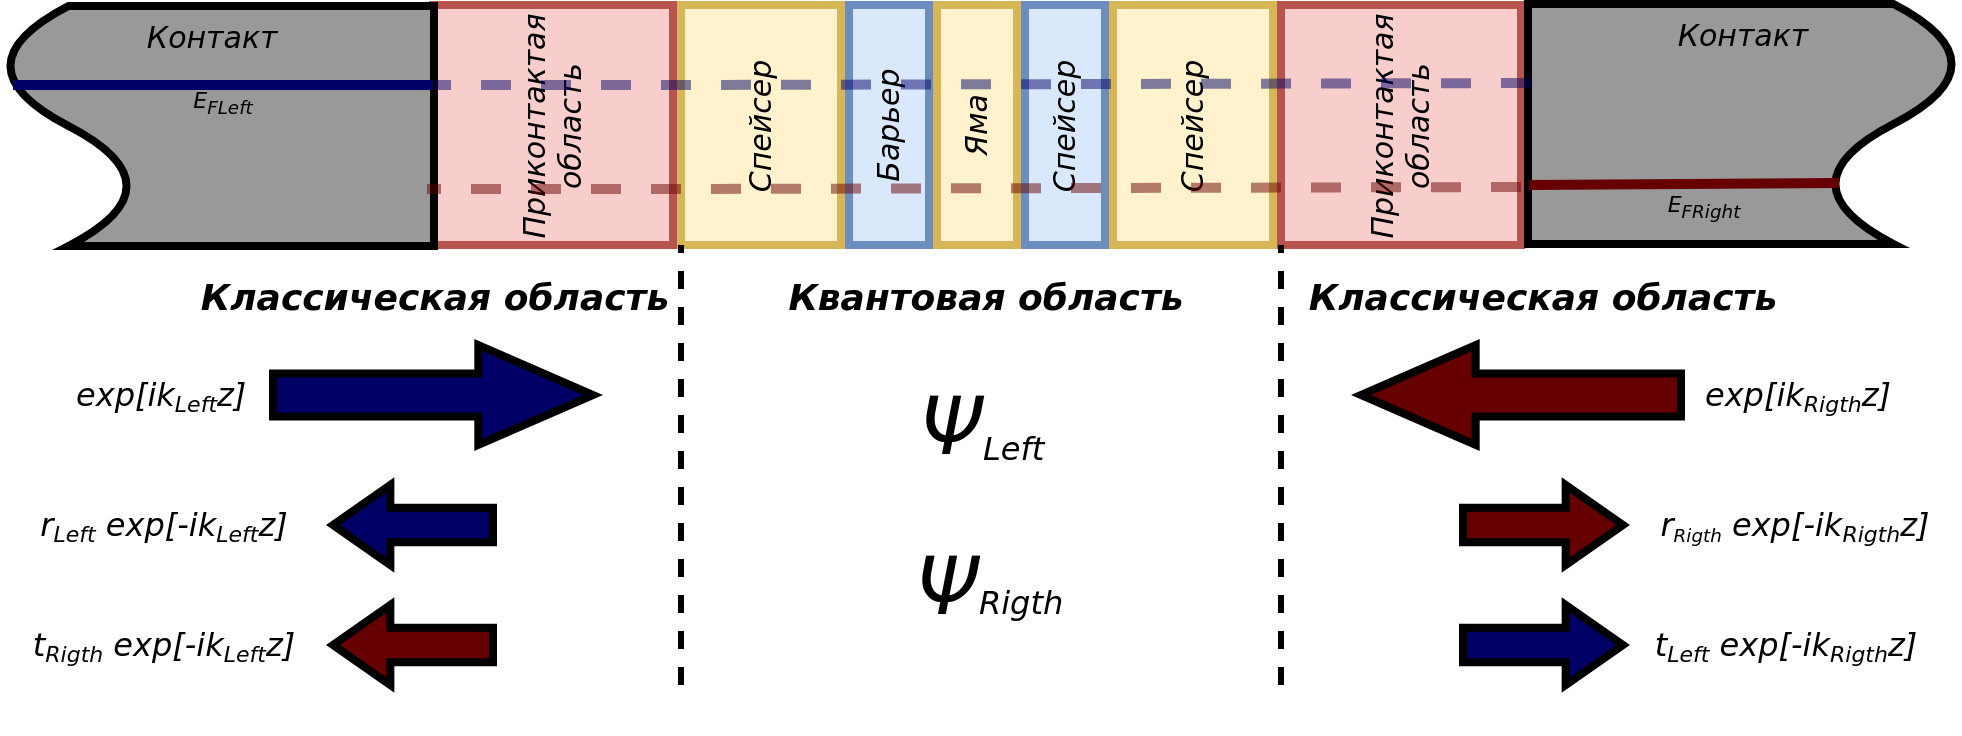
\includegraphics[width=1.08\linewidth]{RTHSModel}
	\caption{Схема модели РТГС}
	\label{fig:RTHSModel}
\end{figure}

Данное схема подходит для любой внутренней точки гетероструктуры, но не подходит для граничных точек. Граничные условия, для <<левых>> и <<правых>> электронов получаются из граничного условия Бастарда и вида волных функций в резервуарах:
\begin{gather}
	\begin{cases}
		(ik_{L}-1)\psi_{1} + \psi_{2} = 2ik_{L}\Delta;\\
		\psi_{N-1} + (ik_{R}\Delta - 1)\psi_{N} = 0;
	\end{cases}\\
	\begin{cases}
		(ik_{L}-1)\psi_{1} + \psi_{2} = 2ik_{L}\Delta;\\
		\psi_{N-1} + (ik_{R}\Delta - 1)\psi_{N} = 0;
	\end{cases}
\end{gather}
\begin{conditions}
	$k_{L(R)}$ & волновые функции в левом (правом) резервуаре.
\end{conditions}
